\documentclass[crop,tikz]{standalone}                 
\usepackage{physics}
\makeatletter                                                                                        

\begin{document}

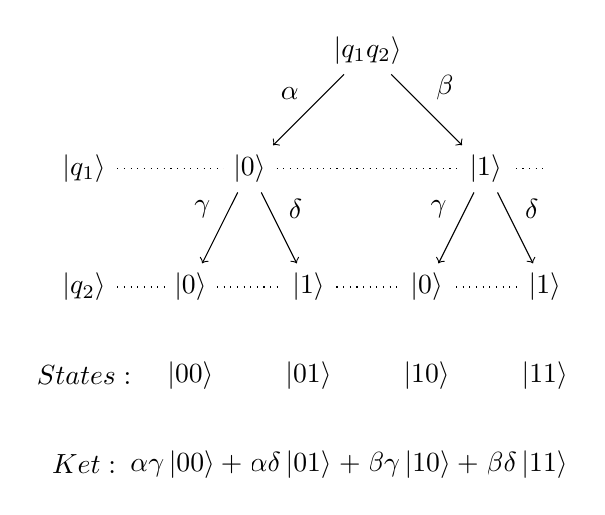
\begin{tikzpicture}[scale=1.5]                                                                          
%\draw [dotted] (0,0) grid (3, 2);

% qubit lines 
\draw [-, dotted] ( -0.90, +0.00) -- ( +3.00, +0.00);
\draw [-, dotted] ( -0.90, +1.00) -- ( +3.00, +1.00);
\node [fill=white] (nodeq1) at ( -0.90, +1.00) {$\ket{q_1}$};                                           
\node [fill=white] (nodeq2) at ( -0.90, +0.00) {$\ket{q_2}$};                                           

% quantum state tree
\node [fill=white] (nodexx) at ( +1.50, +2.00) {$\ket{q_1q_2}$};                                           
\node [fill=white] (node0x) at ( +0.50, +1.00) {$\ket{0}$}     ;                                           
\node [fill=white] (node1x) at ( +2.50, +1.00) {$\ket{1}$}     ;                                           
\node [fill=white] (node00) at ( +0.00, +0.00) {$\ket{0}$}     ;                                          
\node [fill=white] (node01) at ( +1.00, +0.00) {$\ket{1}$}     ;                                          
\node [fill=white] (node10) at ( +2.00, +0.00) {$\ket{0}$}     ;                                          
\node [fill=white] (node11) at ( +3.00, +0.00) {$\ket{1}$}     ;                                       

\draw [->] (nodexx) -- (node0x) node[midway, above left  ] {$\alpha$};                                                           
\draw [->] (nodexx) -- (node1x) node[midway, above right ] {$\beta$ };                                                           
\draw [->] (node0x) -- (node00) node[midway, above left  ] {$\gamma$};                                                           
\draw [->] (node0x) -- (node01) node[midway, above right ] {$\delta$};                                                           
\draw [->] (node1x) -- (node10) node[midway, above left  ] {$\gamma$};                                                           
\draw [->] (node1x) -- (node11) node[midway, above right ] {$\delta$};                                                           

% states / configurations
\node [fill=white] (nodess) at ( -0.90, -0.75) {$States:$} ;                                           
\node [fill=white] (nodes1) at ( +0.00, -0.75) {$\ket{00}$};                                           
\node [fill=white] (nodes2) at ( +1.00, -0.75) {$\ket{01}$};                                           
\node [fill=white] (nodes3) at ( +2.00, -0.75) {$\ket{10}$};                                           
\node [fill=white] (nodes4) at ( +3.00, -0.75) {$\ket{11}$};                                           

% ket state
\node [fill=white] (nodeps) at ( -0.90, -1.50) {$Ket:$}                  ;
\node [fill=white] (nodeaa) at ( -0.15, -1.50) {$\alpha \gamma \ket{00}$};                                          
\node [fill=white] (nodebb) at ( +0.85, -1.50) {$\alpha \delta \ket{01}$};                                          
\node [fill=white] (nodecc) at ( +1.85, -1.50) {$\beta  \gamma \ket{10}$};                                          
\node [fill=white] (nodedd) at ( +2.85, -1.50) {$\beta  \delta \ket{11}$};                                       
\node [fill=white] (nodep1) at ( +0.35, -1.50) {$+$}                     ;
\node [fill=white] (nodep2) at ( +1.35, -1.50) {$+$}                     ;
\node [fill=white] (nodep3) at ( +2.35, -1.50) {$+$}                     ;   
 
\end{tikzpicture}                                                                                    

\end{document}
